\documentclass{standalone}
\usepackage{tikz}
\usepackage{ctex,siunitx}
\setCJKmainfont{Noto Serif CJK SC}
\usepackage{tkz-euclide}
\usepackage{amsmath}
\usetikzlibrary{patterns, calc,3d}
\usetikzlibrary {decorations.pathmorphing,decorations.pathreplacing,decorations.shapes}
\tikzset{label style/.append style={font=\small}}
\begin{document}
\small
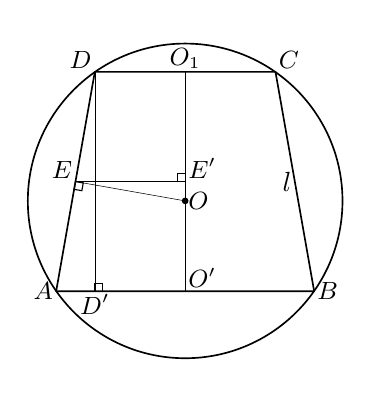
\begin{tikzpicture}[>=latex,scale=1.0,inner sep=1pt]
  \useasboundingbox(-2,-2.2)rectangle(2,2.2);
  \tkzDefPoints{0/0/O}
  \tkzDefPoint(-35:2){B}
  \tkzDefPoint(55:2){C}
  \tkzDefPoint(125:2){D}
  \tkzDefPoint(-145:2){A}
  \tkzDefMidPoint(C,D)\tkzGetPoint{O1}
  \tkzDefMidPoint(A,B)\tkzGetPoint{O'}
  \tkzDefPointsBy[projection=onto A--B](D){D'}
  \tkzDefPointsBy[projection=onto A--D](O){E}
  \tkzDefPointsBy[projection=onto O--O'](E){E'}
  \tkzDrawPolygon[semithick](A,B,C,D)
  \tkzDrawSegments(D,D' O1,O' O,E E,E')
  \tkzDrawPoints[fill=black](O)
  \tkzDrawCircle[semithick,black](O,A)
  \tkzLabelLine[pos=0.5,left](B,C){$l$}
  \tkzLabelPoints[left](A)
  \tkzLabelPoints[below](D')
  \tkzLabelPoints[above left](D,E)
  \tkzLabelPoints[right](B,O)
  \tkzLabelPoint[above](O1){$O_1$}
  \tkzLabelPoints[above right](C,O',E')
  \tkzMarkRightAngle[size=0.1](A,E,O)
  \tkzMarkRightAngle[size=0.1](E,E',O1)
  \tkzMarkRightAngle[size=0.1](D,D',B)
\end{tikzpicture}
\end{document}